\newcommand{\todo}[1]{{\bf TODO} #1}
\newif\ifPAPER  
%\PAPERtrue % select either slide or note
\PAPERfalse  

\def\t{\title{INCL intra-nuclear cascade development for Geant4}}

\def\a{
\author{P.~Kaitaniemi}
\affiliation{CEA/Saclay}
}

\newcommand{\codeAlgorithm}[1]{
\addcontentsline{toc}{section}{Résumé}
\begin{center}\fbox{\parbox{12cm}{\bf #1}}\end{center}}

\newcommand{\cppintro}[1]{
\lstset{language=C,
caption= #1 ,
label=listing:boundary}}

\def\cppstart{\begin{lstlisting}}
\def\cppend{\end{lstlisting}}

\newif\ifCITENOTE 
\CITENOTEtrue

\ifPAPER

\else   % Slides ---------------------------------------------------------------

\documentclass[slidestop,compress,xdvips,10pt]{beamer} 
\usetheme{Antibes}
\usecolortheme{lily}
\usepackage{graphicx}
\usepackage{hyperref}
\usepackage{listings}
\usepackage{verbatim} % for comment
\transglitter[direction=315]
\xdefinecolor{ahcol}{rgb}{0.2, 0.4, 0.1}
\xdefinecolor{olive}{cmyk}{0.64,0,0.95,0.4}
\colorlet{structure}{green!60!black} % for color substitution
\usepackage{color} % for definecolor
\definecolor{light-gray}{gray}{0.95}
\definecolor{dark-gray}{gray}{0.30}
\definecolor{orange}{rgb}{1,0.5,0}
\definecolor{dark-blue}{cmyk}{1,0.5,0.5,0}
%\usepackage{attachfile} 
\hypersetup{
    a4paper, % page format
    pdftitle={My Title},                  % Title
    pdfsubject={Subject of the document}, % Subject 
    pdfauthor={Author name},              % Author
    pdfkeywords={list of keywords},       % Keywords
    plainpages=true, %
    colorlinks,       % links are colored
    urlcolor=dark-blue,    % color of external links
    linkcolor=dark-blue,    % color of internal links
    citecolor=black,  % color of links to bibliography
    bookmarksnumbered
}

\usecolortheme[named=ahcol]{structure}
\useoutertheme{myinfolines}
\useinnertheme{rounded}
\setbeamercolor{alerted_text}{fg=blue}

\makeatother
\beamertemplatetransparentcoveredhigh
\t
\author{Pekka Kaitaniemi\footnote{pekka.kaitaniemi@cea.fr} \\
\vskip1.0cm
CEA/Saclay, SPhN \\
Helsinki Institute of Physics \\
Geant4 Collaboration}

\graphicspath{{.}{figures/}}
\graphicspath{{images/}}
\begin{document}

\frame{\titlepage}

\section{}
\subsection{}
\frame{
\frametitle{INCL, Li\'{e}ge intra-nuclear cascade}
\begin{minipage}{1.0\textwidth}
\begin{minipage}{0.5\textwidth}
\begin{table}
\begin{tabular}{ll}
\hline
Projectile & $p$, $n$, $\pi$, \\
           & deuteron, triton, \\
           & He3, alpha \\
Energy range & 150 MeV - 3 GeV \\
Target nuclei & Carbon - Uranium \\
\hline
\end{tabular}
\caption{Model validity range}
\end{table}
\vskip2mm
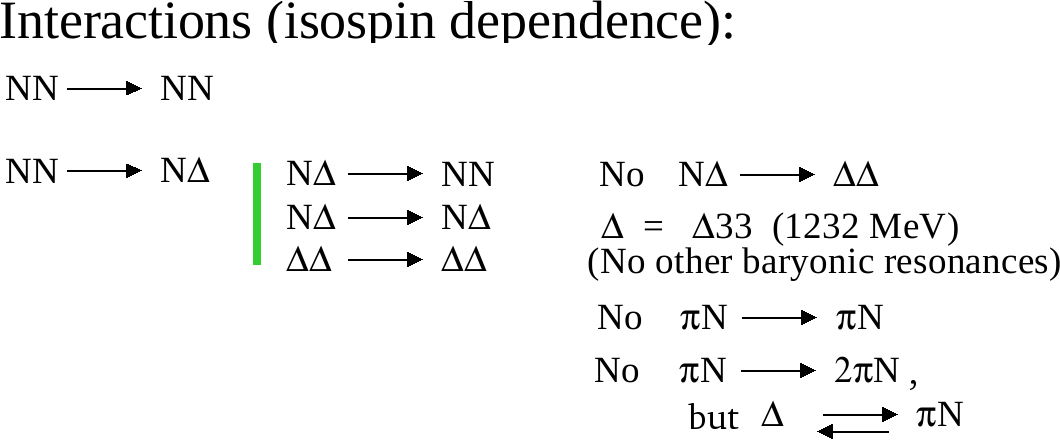
\includegraphics[width=1.0\textwidth]{interactions}
\end{minipage}
\begin{minipage}{0.5\textwidth}
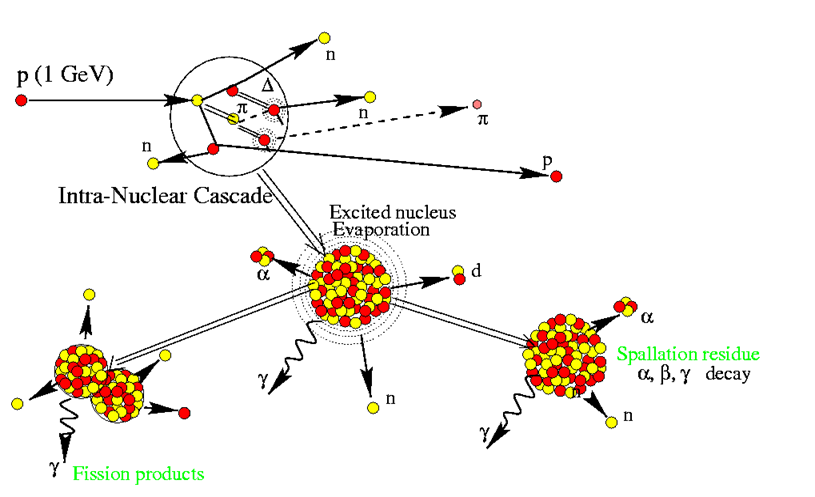
\includegraphics[width=1.0\textwidth]{inclSchematic}
\vskip2mm
\begin{itemize}
\item INCL~\footnote{A. Boudard, C. Volant, S. Leray, J.C. David (CEA/SPhN),
  J. Cugnon, T. Aoust, P. Henrotte (Univ. Li\'{e}ge - Belgium)}
  tracks particles explicitly in time.
\item Stop the cascade when stopping time $t_{stop} = 70.0~\mathrm{fm/c}~(A/208)^{0.16}$ is
  reached.
\end{itemize}
\end{minipage}
\end{minipage}
}

\frame{
\frametitle{Double-differential neutron energy spectra}
\begin{minipage}{1.0\textwidth}
\begin{minipage}{0.5\textwidth}
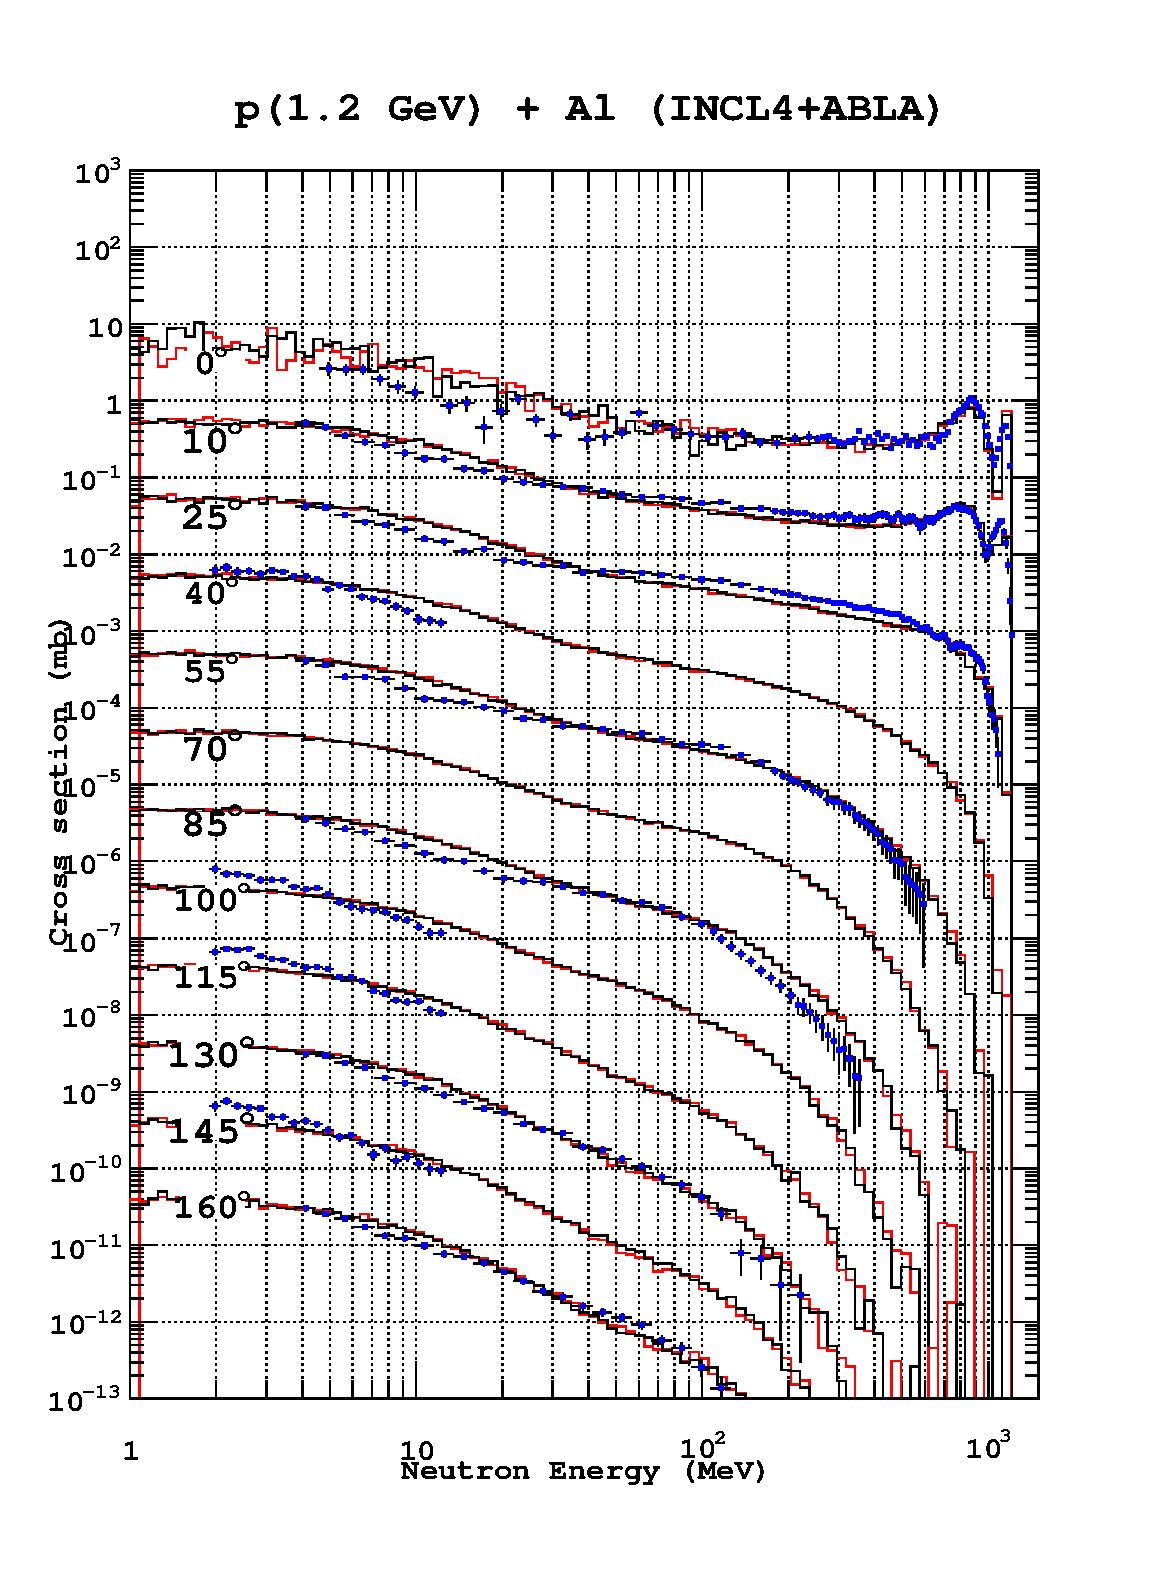
\includegraphics[width=1.0\textwidth]{proton1200MeVAl}
\end{minipage}
\begin{minipage}{0.5\textwidth}
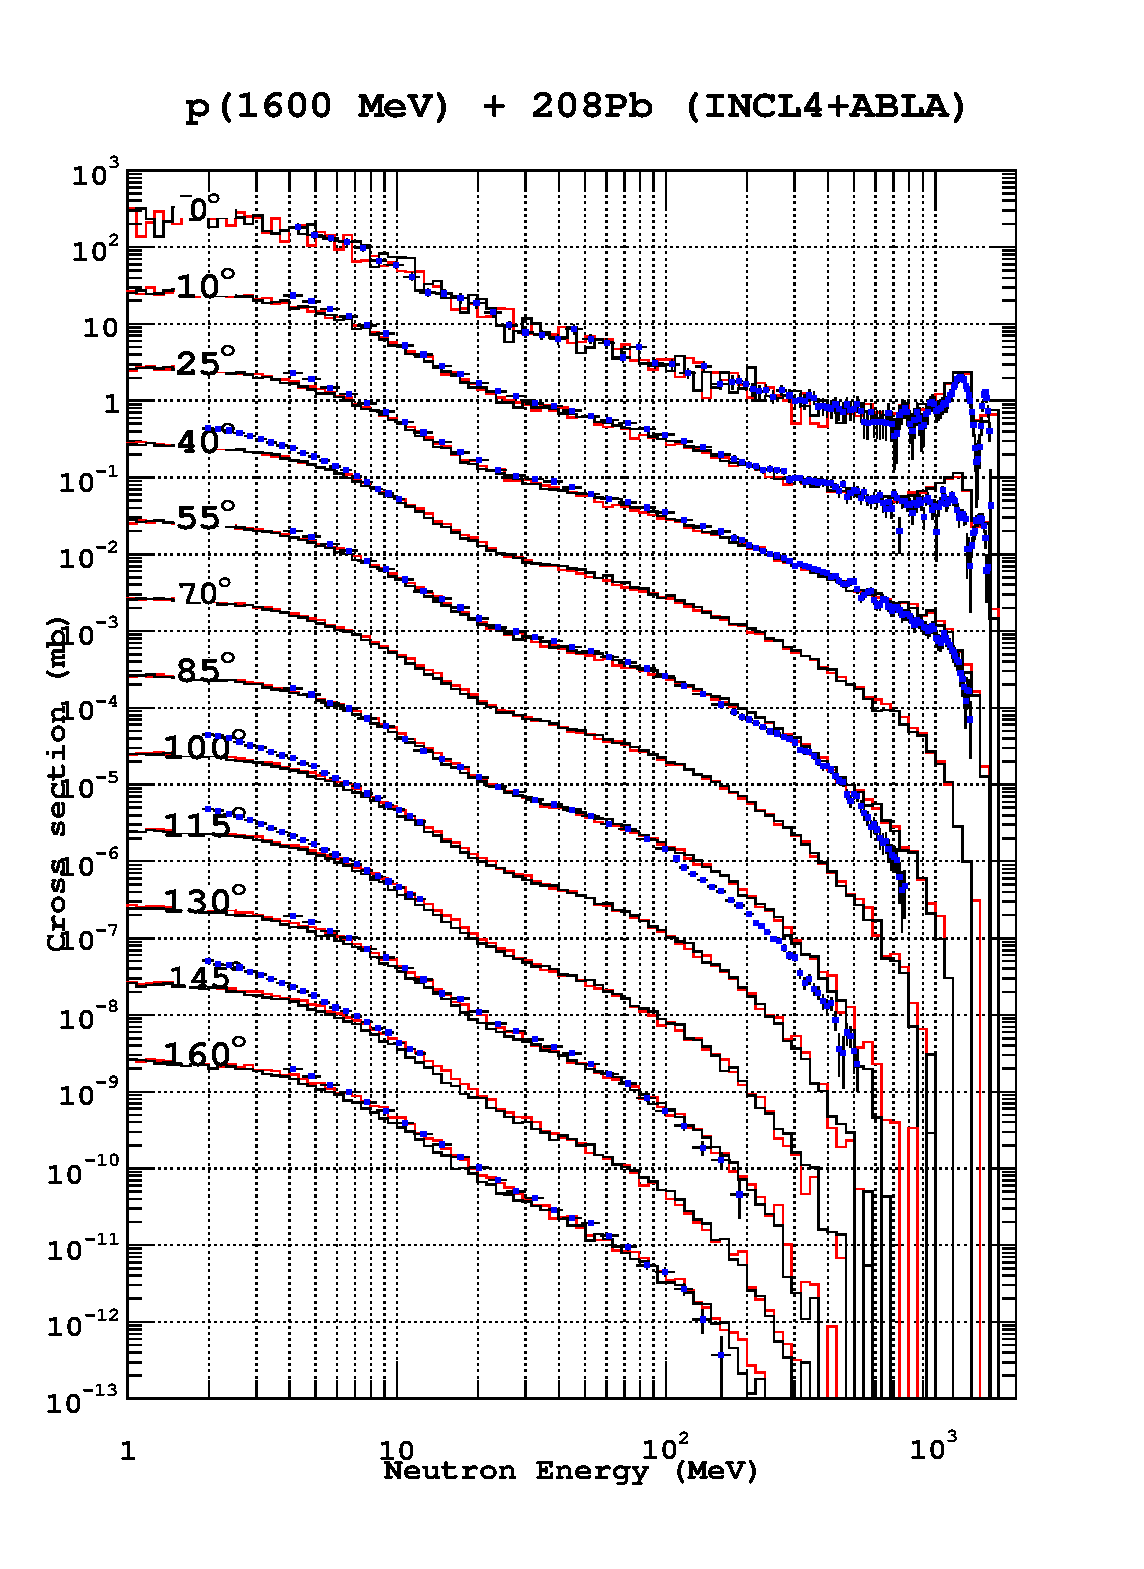
\includegraphics[width=1.0\textwidth]{proton1600MeVPb}
\end{minipage}
\end{minipage}
}

\frame{
\frametitle{Geant4 - Geometry and Tracking}
\vskip0.7cm
\begin{minipage}{1.0\textwidth}
\begin{minipage}{0.6\textwidth}
\begin{itemize}
\item Toolkit for the simulation of the passage of particles through matter
\item Sophisticated geometry system: scales from a simple thick target
  to the description of the LHC detectors
\item Originally a high energy physics toolkit, now used also by
  many space, medical and nuclear physics users
\item Electromagnetic physics
\item Hadronic physics: many models, including INCL
\item Visualization (OpenGL 3D, etc.)
\end{itemize}
\end{minipage}
\begin{minipage}{0.4\textwidth}
\begin{figure}
\caption{Human phantom}
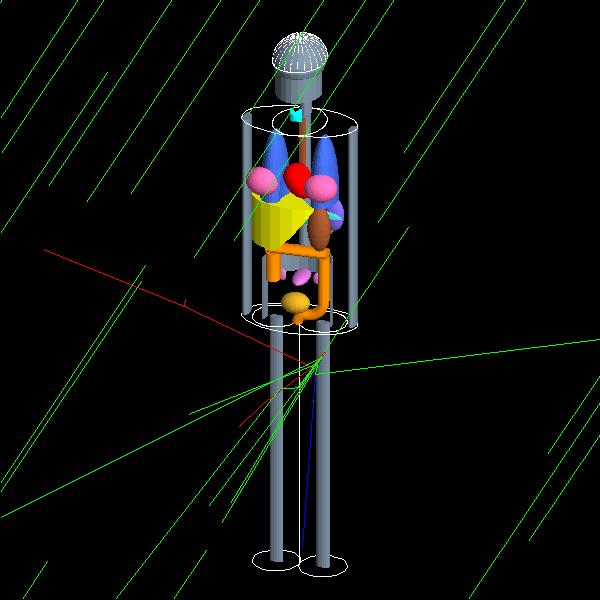
\includegraphics[width=1.0\textwidth]{humanphantom}
\end{figure}
\end{minipage}
\end{minipage}
}

\end{document}

\fi %slides



